\section{Ziel}
Das Ziel des Versuchs ist es, die $\gamma$-Absorptionskurven und -Koeffizienten für Cu, Zn, Fe oder Pb sowie die $\beta$-Absorptionskurve von Al zu ermitteln.

\section{Theorie}
\label{sec:Theorie}
\subsection{Wirkungsquerschnitt und Absorptiongesetz}
Bei der Absorption von $\gamma$- und $\beta$-Strahlung gibt es überschneidene Begrifflichkeiten.\\
Dazu gehört der Wirkungsquerschnitt $\sigma$, der die Häufigkeit dafür darstellt, dass ein Teilchen mit einem Absorbermaterial wechselwirkt. Die Wahrscheinlichkeit dafür, dass das Teilchen eine Reaktion mit dem Absorbermaterial auslöst ist
\begin{equation*}
  W=\frac{nFD\sigma}{F}=nD\sigma,
\end{equation*}
wobei $F$ der Querschnitt, $D$ die Dicke und $n$ die Anzahl der Materieteilchen pro Volumen des Absorbers darstellt und $\sigma$ der Wirkungsquerschnitt dessen. 
Damit ergibt sich bei einem eintreffen von $N_0$ Teilchen pro Zeiteinheit auf der Fläche $F$ ergibt sich zur Berechnung der Wechselwirkungen pro Zeiteinheit 
\begin{equation*}
  N=N_0 nD\sigma
\end{equation*}
für das einfallende Teilchen.\\
Für einen realen Absorber kann unter der Annahme, dass das Teilchen nur einmal mit dem Absorber wechselwirkt, das exponentielle Absorptionsgesetz
\begin{equation}
  N(D)=N_0 e^{-\mu D}
  \label{eq:1}
\end{equation}
verwendet werden, wobei 
\begin{equation}
  \mu=n\sigma
  \label{eq:2}
\end{equation}
der Absorptionskoeffizient ist mit $[\mu]=\frac{1}{\textrm{m}}$.\\
Mit 
\begin{equation*}
  D_{1/2}=\frac{\ln{2}}{\mu}
\end{equation*}
existiert eine gewisse Schichtdicke $D_{1/2}$, bei der sich die Intensität der Strahlung im Mittel halbiert hat. Die Anzahl $n$ der sich stoßenden Teilchen im Absorber pro Volumeneinheit lässt sich durch
\begin{equation}
  n= \frac{z N_{L}}{V_{mol}}= \frac{z N_{L} \rho}{M}
  \label{eq:3}
\end{equation}
beschreiben, wobei $N_{L}$ die Loschmidtsche Zahl, $z$ die Ordnungszahl, $V_{mol}$ das Molvolumen, $M$ das Molekulargewicht und $\rho$ die Dichte des Absorberatoms ist. Wird \eqref{eq:2} in \eqref{eq:3} eingesetzt, ergibt sich 
\begin{equation}
  \sigma=\frac{\mu M}{z N_{L}\rho}
  \label{eq:4}
\end{equation}
diese Abhängigkeit \cite{sample}.

\subsection{Wechselwirkung von Gamma-Strahlung mit Materie}
Wenn ein Atomkern in einen energetisch günstigeren Zustand fällt, dann emittiert dieser einen $\gamma$-Quant. $\gamma$-Strahlung besitzt typische Eigenschaften einer elektromagnetischen Welle. Deshalb kann die Energie mit der Quantentheorie durch
\begin{equation*}
  E_{\gamma}=\frac{hc}{\lambda}
\end{equation*}
dargestellt werden, wobei $h$ das Plancksche Wirkumsquantum, $c$ die Lichtgeschwindigkeit und $\lambda$ die Wellenlänge darstellt. Da die Energieniveaus der Kerne genau definiert sind, ist das $\gamma$-Linienspektrum extrem scharf darstellbar. \\
Das $\gamma$-Quant emittiert üblicherweise in den Energiebereichen $10$ keV bis $10$ MeV. In diesem Bereich treten diese drei signifikante Prozesse häufig auf:
\begin{enumerate}[nosep,label=\textsc{\arabic*},leftmargin=*]
\item (innerer) Photoeffekt: Das $\gamma$-Quant wechselwirkt mit einem Hüllenelektron und wird vom Hüllenelektron absorbiert, das dann aus der Bindung gelöst wird. Da das Elektron bei diesem Vorgang kinetische Energie erhält, ist der Photo-Effekt von einer Energieschwelle abhängig. Ist $E_{Bindung}>E_\gamma$, dann findet der Effekt nicht statt. Der Stoß ist für festgebundene Elektronen wahrscheinlicher, weshalb meistens die Elektronen aus der innersten Schale gelöst werden, wodurch wieder Röntgenquanten oder Auger-Elektronen emittiert werden. Der Wirkungsquerschnitt ist in diesem Fall proportional zu $z^5$ und $E_\gamma^{-3.5}$.
\item Compton-Effekt: Beim Compton-Effekt stößt ein Photon an ein ruhendes Elektron und beide (Quasi-)Teilchen ändern ihre Richtung und Energie. Das Photon gibt dabei Energie an das Elektron ab, wird dabei aber nicht zerstört. Das führt zu einer Senkung der Intensität eines $\gamma$-Strahls, da die Quanten in verschiedene Richtung abgelenkt werden. Nach Klein und Nishina ist der Wirkungsquerschnitt
\begin{equation}
  \sigma_{COM} = 2\pi r_e^2\left\{\frac{1+\epsilon}{\epsilon^2}\left[\frac{2(1+\epsilon)}{1+2\epsilon}-\frac{1}{\epsilon}\ln(1+2\epsilon)\right]+\frac{1}{2\epsilon}\ln(1+2\epsilon)-\frac{1+3\epsilon}{(1+2\epsilon)^2}\right\} 
  \label{eqlig}
\end{equation}
abhängig von dem klassischen Radius $r_e=2.82\cdot 10^{-15}$ m des Elektrons und dem Verhältnis 
\begin{equation*}
  \epsilon=\frac{E_\gamma}{m_e c^2}
\end{equation*} 
der Photonenenergie $E_\gamma$ und der Ruheenergie $m_e c^2$ des Elektrons.\\
Da der Compton-Effekt so beschrieben wird, dass er quasi aus einem Stoß freier Teilchen resultiert, ist der Wirkungsquerschnitt abhängig von $z$. Dadurch lässt sich der Absorptionskoeffizient $\mu_{com}$ durch
\begin{equation}
  \mu_{com}=\frac{zN_L \rho}{M}\sigma_{com}
  \label{eqlig2}
\end{equation}
beschreiben. 
\item Paarbildung: Ist die Energie des Photons größer als die doppelte Ruhemasse des Elektrons, dann kann das Gamma-Quant durch die Erzeugung eines Positron-Elektron-Paars annihiliert werden. Um die Impulserhaltung zu erfüllen, muss allerdings ein weiterer Stoßpartner für das Photon existieren. Diese finden sich in der Nähe des Atomkerns, der bestrahlt wird. Der Wirkungsquerschnitt ist proportional zu $z^2$.
\end{enumerate}
Durch diese sich überlagernden Effekte entsteht eine komplizierte Kurve, die für das Beispiel Germanium in \autoref{1} abgebildet wird. 
\begin{figure}[H]
    \centering
    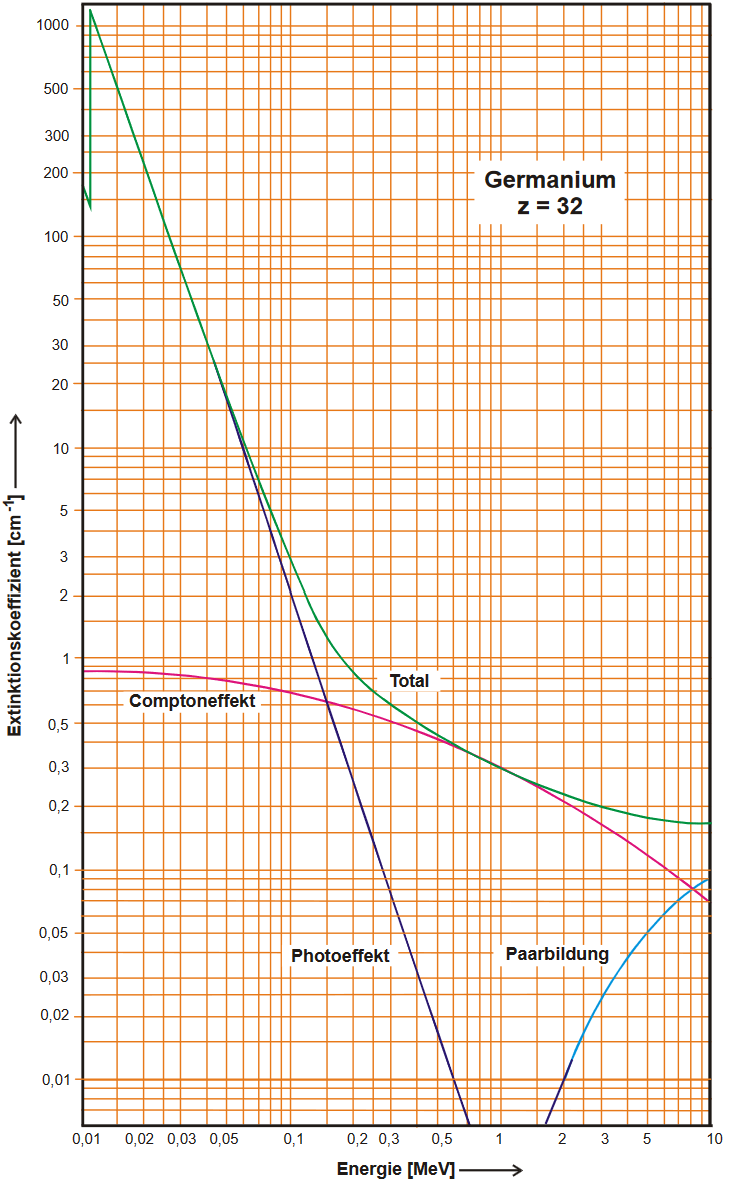
\includegraphics[width = 9cm]{content/1}
    \caption{Überlagerung der Effekte in Germanium \cite{sample}.}
    \label{1}
\end{figure}
Der Photoeffekt findet bis 200 keV statt, dann setzt der Compton-Effekt ein, der bis 1 MeV dominiert. Ab 100 MeV findet fast nur Paarbildung statt \cite{sample}. 

\subsection{Wechselwirkung von Beta-Strahlung mit Materie}
Bei instabilen Atomkernen zerfällt der Kern, indem er ein überschüssiges Neutron oder Proton emittiert. Die Reaktionskette wird durch
\begin{align*}
  n &\rightarrow p+\beta^- + \bar\nu_e\\
  p &\rightarrow n+\beta^+ + \nu_e
\end{align*}
beschrieben. Wegen der Ladungserhaltung ist der $\beta$-Strahl geladen. Dieser ist entweder ein Elektron- oder Positron-Jet. Da sich die Energie des Prozesse auf die Nebenteilchen verteilt, entsteht ein kontinuierliches Energiespektrum für den $\beta$-Strahler. Das Maximum des Spektrums ist die freiwerdende Energie durch den Kernumwandlungsprozess. Es gibt drei wichtige Wechselwirkungen:
\begin{enumerate}[nosep,label=\textsc{\arabic*},leftmargin=*]
\item Elastische Streuung am Atomkern:\\
Diese Wechselwirkung wird auch Rutherford-Streuung genannt. Diese ist dadurch charakterisiert, dass das $\beta$-Teilchen elastisch an dem Atomkern streut. Das passiert durch die Umlenkung des Teilchens durch das elektrische Feld des Kerns. Dadurch verringert sich die Intensität des Strahls. Die Energieabnahme ist gering, die Richtungsänderung jedoch signifikant. 
\item Inelastische Streuungen an Atomkernen des Absorbermaterials:\\
Befindet sich das $\beta$-Teilchen in einem elektrischen Feld, dann wird es beschleunigt. Durch diese Beschleunigung absorbiert oder emittiert es Photonen. Die Strahlung, die zum Bremsen des Teilchens führt, heißt Bremsstrahlung. Die Wahrscheinlichkeit der Bremsstrahlung ist durch den Wirkungsquerschnitt
\begin{equation*}
  \sigma_{Br}=\alpha r_e^2\cdot z^2
\end{equation*}
gegeben, mit der Sommerfelschen Feinstrukturkonstante $\alpha=\frac{1}{137}$.\\
Die Energie, die bei der Bremststrahlung verloren geht wird durch 
\begin{equation*}
  E_{Br}\approx 7\cdot 10^{-7}zE_{\beta}^2
\end{equation*}
beschrieben, wobei $E_\beta$ die Energie des einfallenden $\beta$-Teilchens ist. 
\item Inelastische Streuung an den Elektronen des Absorbermaterials:\\
Bei diesem Prozess werden die Absorberatome ionisiert und angeregt. Hierbei wird wenig Energie des $\beta$-Teilchens benötigt, sodass es zu mehreren dieser Prozesse kommen kann. Der Energieverlust pro Absorberschichtdicke ist durch
\begin{equation*}
  \frac{\textrm{d}E}{\textrm{d}x}=-\frac{2\pi r_e^2}{E_\beta}\frac{N_L \rho}{M}z\ln(\frac{E_\beta}{I})
\end{equation*}
gegeben, wobei $I=3.13\cdot 10^{-5}\cdot z^{0.9}$ die Ionisationsenergie der Absorberatome beschreibt. 
\end{enumerate}
Die Gestalt der Absorptionskurve ist in \autoref{2} dargestellt. 
\begin{figure}[H]
    \centering
    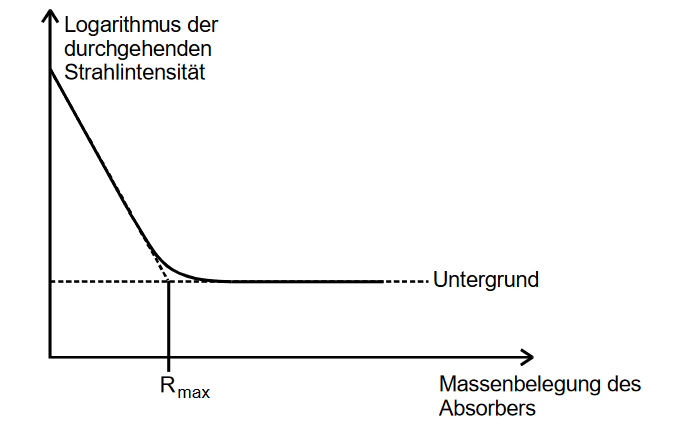
\includegraphics[width = 9cm]{content/2}
    \caption{Absorptionsspektrum eines $\beta$-Strahlers \cite{sample}.}
    \label{2}
\end{figure} 
Dort ist statt der Schichtdicke $D$ die Massenbelegung $R$ des Absorbers auf der x-Achse aufgetragen. Diese hängen durch
\begin{equation*}
  R=\rho D
\end{equation*}
zusammen. Die Absorptionskurve aus \autoref{2} kann genutzt werden, um die maximale Reichweite der $\beta$-Teilchen zu bestimmen. Dafür gilt in diesem Experiment der Zusammenhang
\begin{equation}
  E_{max}=1.92\cdot\sqrt{R_{max}^2+0.22\cdot R_{max}}
  \label{energie}
\end{equation}
zwischen der maximalen Energie $E_{max}$ und der maximalen Reichweite $R_{max}$ \cite{sample}.
